\documentclass[12pt,letterpaper]{article}
\usepackage{graphicx,textcomp}
\usepackage{natbib}
\usepackage{setspace}
\usepackage{fullpage}
\usepackage{color}
\usepackage[reqno]{amsmath}
\usepackage{amsthm}
\usepackage{fancyvrb}
\usepackage{amssymb,enumerate}
\usepackage[all]{xy}
\usepackage{endnotes}
\usepackage{lscape}
\newtheorem{com}{Comment}
\usepackage{float}
\usepackage{hyperref}
\newtheorem{lem} {Lemma}
\newtheorem{prop}{Proposition}
\newtheorem{thm}{Theorem}
\newtheorem{defn}{Definition}
\newtheorem{cor}{Corollary}
\newtheorem{obs}{Observation}
\usepackage[compact]{titlesec}
\usepackage{dcolumn}
\usepackage{tikz}
\usetikzlibrary{arrows}
\usepackage{multirow}
\usepackage{xcolor}
\newcolumntype{.}{D{.}{.}{-1}}
\newcolumntype{d}[1]{D{.}{.}{#1}}
\definecolor{light-gray}{gray}{0.65}
\usepackage{url}
\usepackage{listings}
\usepackage{color}
\usepackage[utf8]{inputenc}
\usepackage{verbatim} % includes comment blocks
%\usepackage{rotating}
%\usepackage{geometry}
%\usepackage{pdflscape}
\usepackage{lscape}

\definecolor{codegreen}{rgb}{0,0.6,0}
\definecolor{codegray}{rgb}{0.5,0.5,0.5}
\definecolor{codepurple}{rgb}{0.58,0,0.82}
\definecolor{backcolour}{rgb}{0.95,0.95,0.92}

\lstdefinestyle{mystyle}{
	backgroundcolor=\color{backcolour},
	commentstyle=\color{codegreen},
	keywordstyle=\color{magenta},
	numberstyle=\tiny\color{codegray},
	stringstyle=\color{codepurple},
	basicstyle=\footnotesize,
	breakatwhitespace=false,
	breaklines=true,
	captionpos=b,
	keepspaces=true,
	numbers=left,
	numbersep=5pt,
	showspaces=false,
	showstringspaces=false,
	showtabs=false,
	tabsize=2
}
\lstset{style=mystyle}
\newcommand{\Sref}[1]{Section~\ref{#1}}
\newtheorem{hyp}{Hypothesis}

\title{Applied Stats II - Problem Set 4}
\date{Due: April 16, 2023}
\author{Imelda Finn (22334657)}

\begin{document}
	\maketitle
\begin{comment}
	\section*{Instructions}
	\begin{itemize}
	\item Please show your work! You may lose points by simply writing in the answer. If the problem requires you to execute commands in \texttt{R}, please include the code you used to get your answers. Please also include the \texttt{.R} file that contains your code. If you are not sure if work needs to be shown for a particular problem, please ask.
	\item Your homework should be submitted electronically on GitHub in \texttt{.pdf} form.
	\item This problem set is due before 23:59 on Sunday April 16, 2023. No late assignments will be accepted.

	\end{itemize}

	\vspace{.25cm}
\end{comment}

	Code in \texttt{PS4\_ImeldaFinn.R}

\section*{Question 1}
\vspace{.25cm}
\noindent We're interested in modeling the historical causes of child mortality. We have data from 26574 children born in Skellefteå, Sweden from 1850 to 1884. Using the ``child" dataset in the \texttt{eha} library, fit a Cox Proportional Hazard model using mother's age and infant's gender as covariates. Present and interpret the output.

%  \lstinputlisting[language=R, firstline=54, lastline=54]{PS4_ImeldaFinn.R}
%===============================================================
  \lstinputlisting[language=R, firstline=63, lastline=65]{PS4_ImeldaFinn.R}
%=============================================================	
The model results are shown in Table~\ref{tbl:add}, and the likelihood ratio test results in Table~\ref{tbl:add:drop}.  %Mother's age is a significant predictor at 0.001 level, child's sex at 0.01 level.  
Base case for sex is male, mean age for mother is 32.

There is a 0.082 decrease in the expected log of the hazard for female babies compared to male, holding mother's age constant. For a unit increase of mother's age, there is a 0.008 increase in the expected log of the hazard, holding sex constant.\footnote{The interaction term for $m.age\times sex$ is 0.001, and is not significant, $p-value =0.7445$}

The hazard ratio of female babies is 0.92 that of male babies, i.e. female babies are less likely to die (92 female babies die for every 100 male babies; female deaths are 8\% lower, etc.), holding mother's age constant.  

  
% Table created by stargazer v.5.2.3 by Marek Hlavac, Social Policy Institute. E-mail: marek.hlavac at gmail.com
% Date and time: Thu, Apr 13, 2023 - 22:23:12
\begin{table}[!htbp] \centering 
  \caption{} 
  \label{} 
\begin{tabular}{@{\extracolsep{5pt}}lc} 
\\[-1.8ex]\hline 
\hline \\[-1.8ex] 
 & \multicolumn{1}{c}{\textit{Dependent variable:}} \\ 
\cline{2-2} 
\\[-1.8ex] & child\_surv \\ 
\hline \\[-1.8ex] 
 m.age & 0.008$^{***}$ \\ 
  & (0.002) \\ 
  & \\ 
 sexfemale & $-$0.082$^{***}$ \\ 
  & (0.027) \\ 
  & \\ 
\hline \\[-1.8ex] 
Observations & 26,574 \\ 
R$^{2}$ & 0.001 \\ 
Max. Possible R$^{2}$ & 0.986 \\ 
Log Likelihood & $-$56,503.480 \\ 
Wald Test & 22.520$^{***}$ (df = 2) \\ 
LR Test & 22.518$^{***}$ (df = 2) \\ 
Score (Logrank) Test & 22.530$^{***}$ (df = 2) \\ 
\hline 
\hline \\[-1.8ex] 
\textit{Note:}  & \multicolumn{1}{r}{$^{*}$p$<$0.1; $^{**}$p$<$0.05; $^{***}$p$<$0.01} \\ 
\end{tabular} 
\end{table}  

  
% Table created by stargazer v.5.2.3 by Marek Hlavac, Social Policy Institute. E-mail: marek.hlavac at gmail.com
% Date and time: Sun, Apr 16, 2023 - 00:46:25
\begin{table}[!htbp] \centering 
  \caption{} 
  \label{tbl:add:drop} 
\begin{tabular}{@{\extracolsep{5pt}}lccccc} 
\\[-1.8ex]\hline 
\hline \\[-1.8ex] 
Statistic & \multicolumn{1}{c}{N} & \multicolumn{1}{c}{Mean} & \multicolumn{1}{c}{St. Dev.} & \multicolumn{1}{c}{Min} & \multicolumn{1}{c}{Max} \\ 
\hline \\[-1.8ex] 
Df & 2 & 1.000 & 0.000 & 1 & 1 \\ 
AIC & 3 & 113,017.100 & 5.528 & 113,011.000 & 113,021.800 \\ 
LRT & 2 & 11.130 & 2.355 & 9.465 & 12.795 \\ 
Pr(\textgreater Chi) & 2 & 0.001 & 0.001 & 0.0003 & 0.002 \\ 
\hline \\[-1.8ex] 
\end{tabular} 
\end{table}  

\clearpage

  \begin{figure}[!htbp]
	  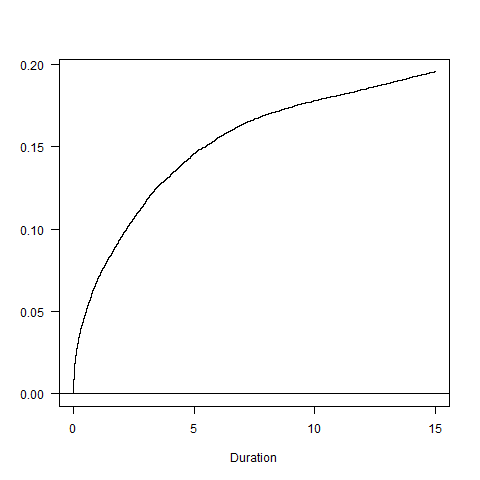
\includegraphics[width=0.7\textwidth,height=0.5\textheight]{graphics/coxreg.png}
	  \caption{Cox Proportional-Hazard}
	  \label{fig:cox}
	\end{figure}



  \begin{figure}[!htbp]
	  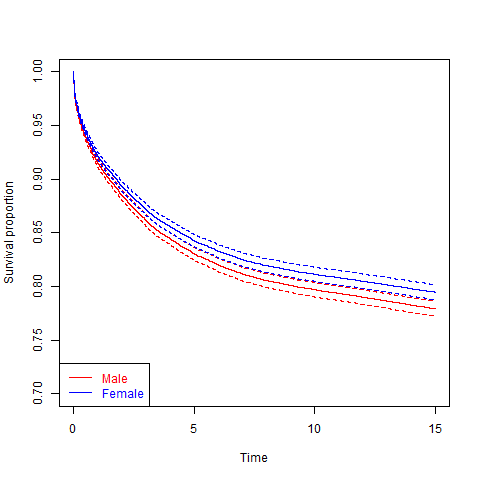
\includegraphics[width=0.85\textwidth]{graphics/surv_prop.png}
	  \caption{survival proportions - m.age = 32}
	  \label{fig:survprop}
	\end{figure}

\begin{comment}  
  \end{comment]



\begin{comment}

  \begin{figure}[!htbp]
	  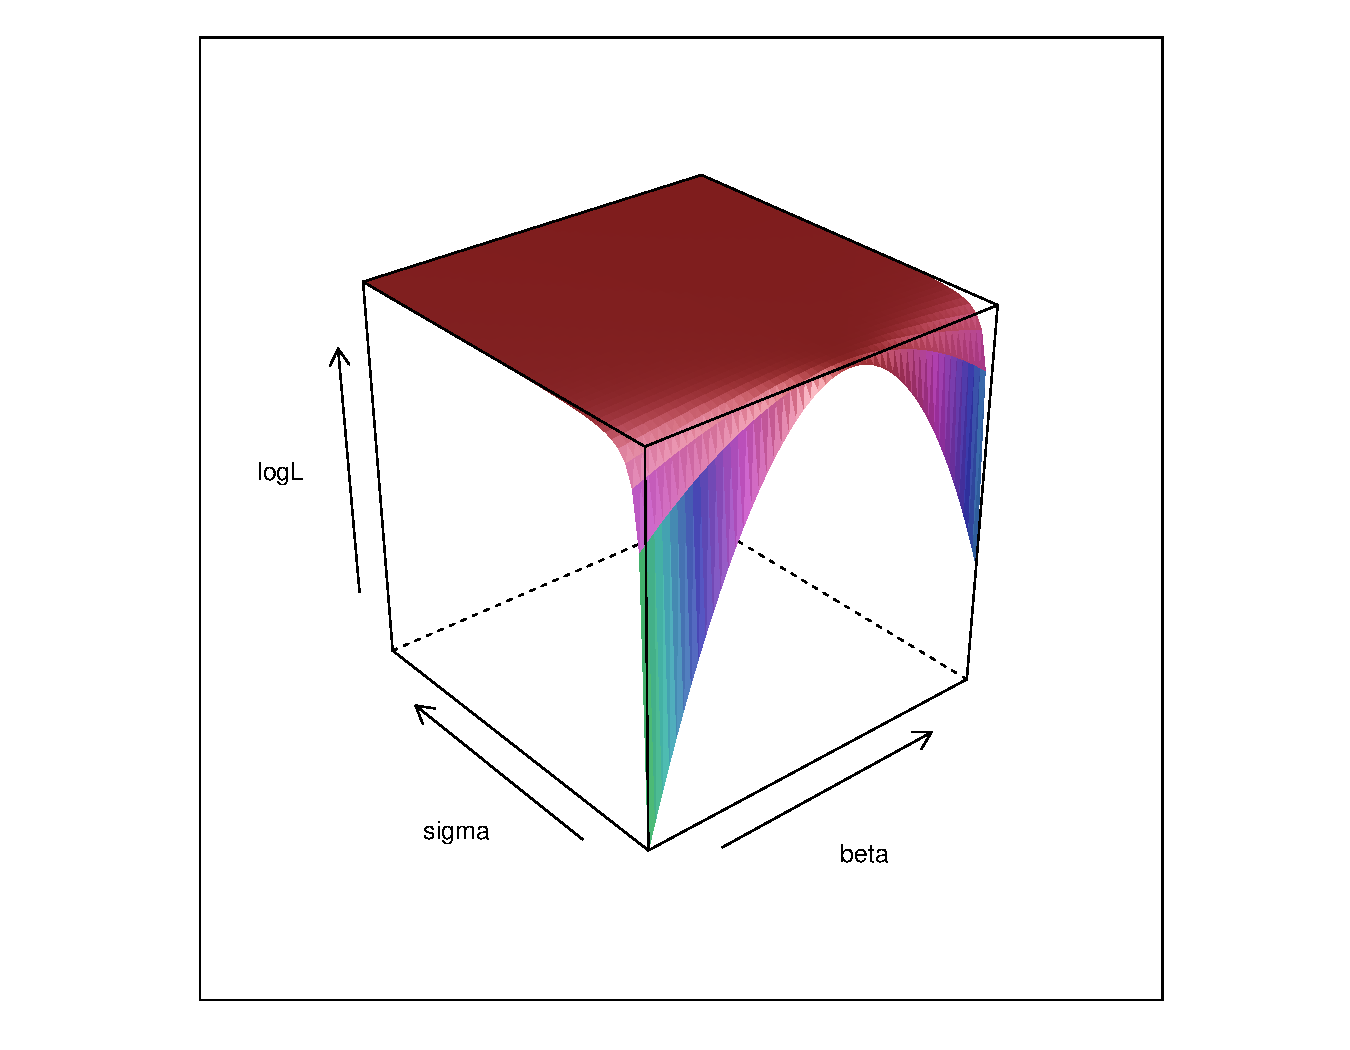
\includegraphics[width=0.7\textwidth]{graphics/wireframe.pdf}
	  \caption{mle surface}
	  \label{fig:surface}
	\end{figure}
  \begin{figure}[!htbp]
	  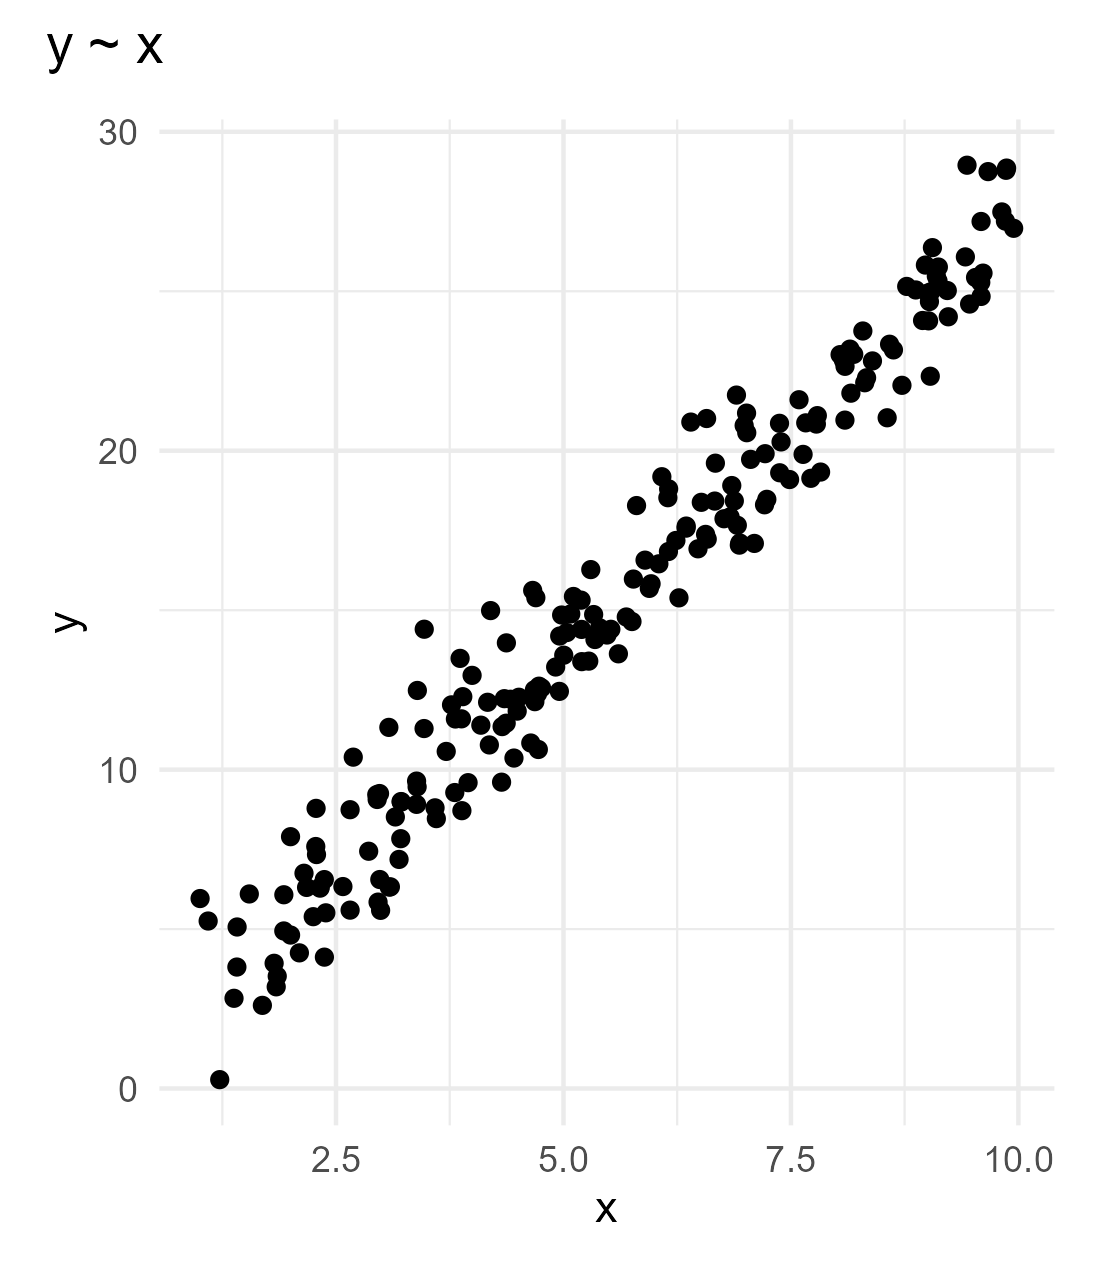
\includegraphics[width=0.7\textwidth]{graphics/q2_xy.png}
	  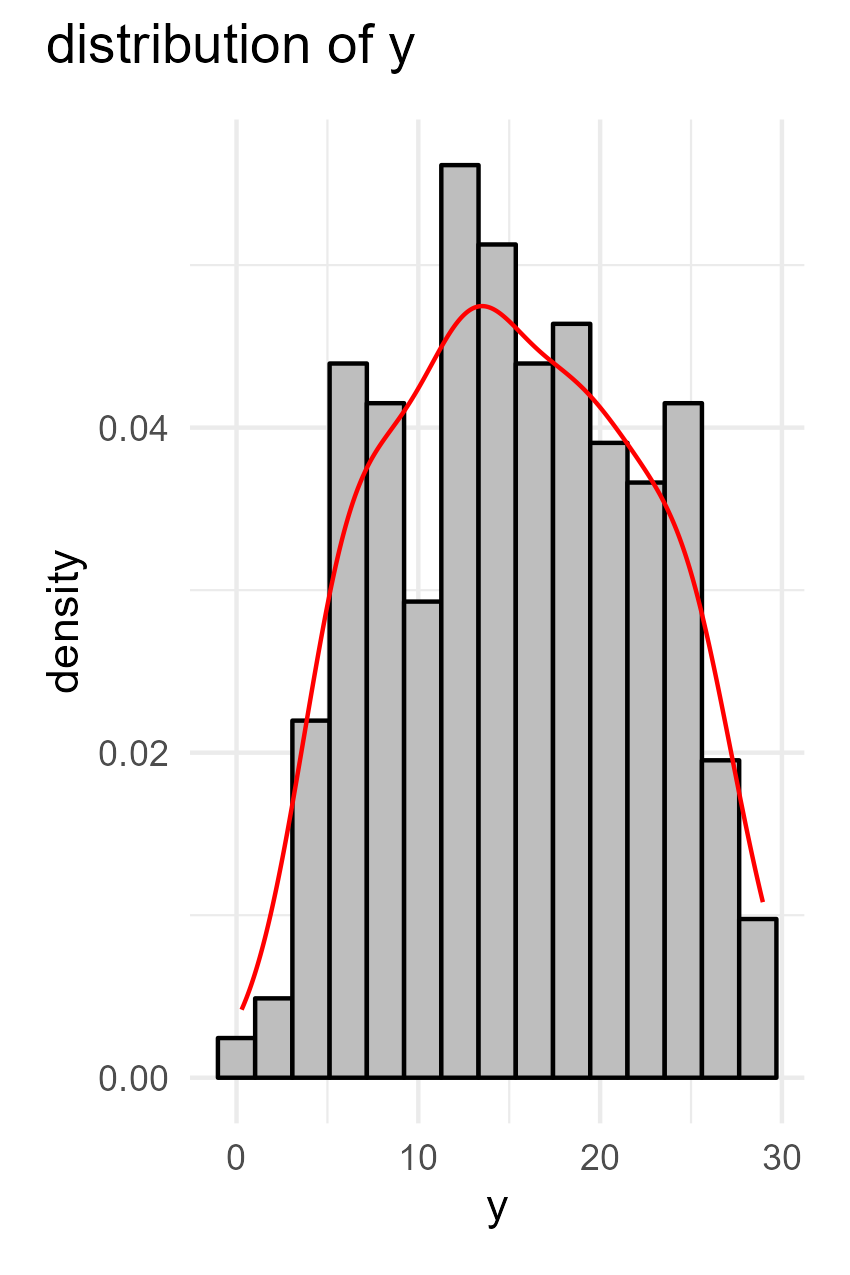
\includegraphics[width=0.7\textwidth]{graphics/q2_hist.png}
	  \caption{Q2 Data}
	  \label{fig:mle}
	\end{figure}

	\clearpage

\lstinputlisting[language=R, firstline=3,lastline=3]{PS3_ImeldaFinn.R}

	The prediction equation is: $y = 0.1398324 + 2.7265559 \times x$.

	$\hat y =  0.13983  (\theta)  +  5.55753  (\bar{x}) *  2.72656  (\beta) =  15.29274$

	$\bar y = 15.29289$
\end{comment}

%https://www.sascha-frank.com/Faq/tables_three.html
%http://www.sthda.com/english/wiki/ggplot2-facet-split-a-plot-into-a-matrix-of-panels#facet-labels
  \begin{comment}
  \begin{lstlisting}[language=R]
  \end{lstlisting}

  \begin{sidewaystable}
%\begin{tabular}...\end{tabular}
  \end{sidewaystable}
  %
% Table created by stargazer v.5.2.3 by Marek Hlavac, Social Policy Institute. E-mail: marek.hlavac at gmail.com
% Date and time: Tue, Mar 21, 2023 - 15:08:02
\begin{table}[!htbp] \centering 
  \caption{} 
  \label{tbl:gdp} 
\begin{tabular}{@{\extracolsep{5pt}} ccccccc} 
\\[-1.8ex]\hline 
\hline \\[-1.8ex] 
GDPWdiff & GDPWdiff & Min / Max & -2506.0 / 2821.0 & -3741.0 / 3722.0 & -9257.0 / 7867.0 & -5997.0 / 3555.0 \\ 
GDPWdiff & GDPWdiff & Med [IQR] & 50.0 [-30.0;215.0] & 293.0 [13.5;644.8] & 140.5 [-50.0;463.0] & 39.0 [-527.2;421.8] \\ 
GDPWdiff & GDPWdiff & Mean (std) & 106.0 (395.3) & 319.4 (561.6) & 141.2 (1147.3) & -46.5 (1228.4) \\ 
GDPWdiff & GDPWdiff & N (NA) & 1939 (0) & 1408 (0) & 288 (0) & 86 (0) \\ 
\hline \\[-1.8ex] 
\end{tabular} 
\end{table} 

% Table created by stargazer v.5.2.3 by Marek Hlavac, Social Policy Institute. E-mail: marek.hlavac at gmail.com
% Date and time: Tue, Mar 21, 2023 - 15:08:02
\begin{table}[!htbp] \centering 
  \caption{} 
  \label{tbl:gdp} 
\begin{tabular}{@{\extracolsep{5pt}} c} 
\\[-1.8ex]\hline 
\hline \\[-1.8ex] 
GDP data summary \\ 
\hline \\[-1.8ex] 
\end{tabular} 
\end{table}  


  \begin{landscape}
    
% Table created by stargazer v.5.2.3 by Marek Hlavac, Social Policy Institute. E-mail: marek.hlavac at gmail.com
% Date and time: Tue, Mar 21, 2023 - 15:08:02
\begin{table}[!htbp] \centering 
  \caption{} 
  \label{tbl:gdp} 
\begin{tabular}{@{\extracolsep{5pt}} ccccccc} 
\\[-1.8ex]\hline 
\hline \\[-1.8ex] 
GDPWdiff & GDPWdiff & Min / Max & -2506.0 / 2821.0 & -3741.0 / 3722.0 & -9257.0 / 7867.0 & -5997.0 / 3555.0 \\ 
GDPWdiff & GDPWdiff & Med [IQR] & 50.0 [-30.0;215.0] & 293.0 [13.5;644.8] & 140.5 [-50.0;463.0] & 39.0 [-527.2;421.8] \\ 
GDPWdiff & GDPWdiff & Mean (std) & 106.0 (395.3) & 319.4 (561.6) & 141.2 (1147.3) & -46.5 (1228.4) \\ 
GDPWdiff & GDPWdiff & N (NA) & 1939 (0) & 1408 (0) & 288 (0) & 86 (0) \\ 
\hline \\[-1.8ex] 
\end{tabular} 
\end{table} 

% Table created by stargazer v.5.2.3 by Marek Hlavac, Social Policy Institute. E-mail: marek.hlavac at gmail.com
% Date and time: Tue, Mar 21, 2023 - 15:08:02
\begin{table}[!htbp] \centering 
  \caption{} 
  \label{tbl:gdp} 
\begin{tabular}{@{\extracolsep{5pt}} c} 
\\[-1.8ex]\hline 
\hline \\[-1.8ex] 
GDP data summary \\ 
\hline \\[-1.8ex] 
\end{tabular} 
\end{table}  

  \end{landscape}

  \end{comment}

\end{document}
